\chapter{Theorie}
\label{cha:Theorie}

\section{Funktionsweise eines Lasers}

Ein Laser (light amplification of stimulated emission of radiation) ist eine gute Quelle für monochromatische kohärente 
elektromagnetische Wellen. Erzeugt werden diese Wellen durch die Anregung eines Mediums und die darauffolgende Emission
von Photonen. Angeregt wird das Lasermedium durch eine Pumpquelle, wodurch eine Besetzungsinversion des Lasermediums erzwungen wird.\\
Bei der darauffolgenden Emission kann zwischen zwei grundlegenden Arten unterschieden werden - eine spontane und eine stimulierte
Emission. Eine spontane Emission der 
Photonen entsteht, wenn ein Atom des angeregten Mediums aus dem energetisch erhöhten Zustand in den Grundzustand zurückfällt und 
ein Photon mit der Energie des Übergangs emittiert. 
Eine weitere Möglichkeit aus den angeregten Zuständen Photonen zu erzeugen, besteht in der stimulierten Emission. Hier wird
das Lasermedium mit Photonen bestrahlt, welche dieselbe Energie aufweisen, wie die der emittierten Photonen. Dadurch werden Photonen emittiert,
welche dieselben Charakteristika (Ausbreitungsrichtung, Energie, Phase und Polarisation) wie die, die zur Emission angeregt haben besitzen. Die spontane und stimulierte 
Emission sind schematisch in \autoref{fig:emission} dargestellt.
\begin{figure}
    \centering
    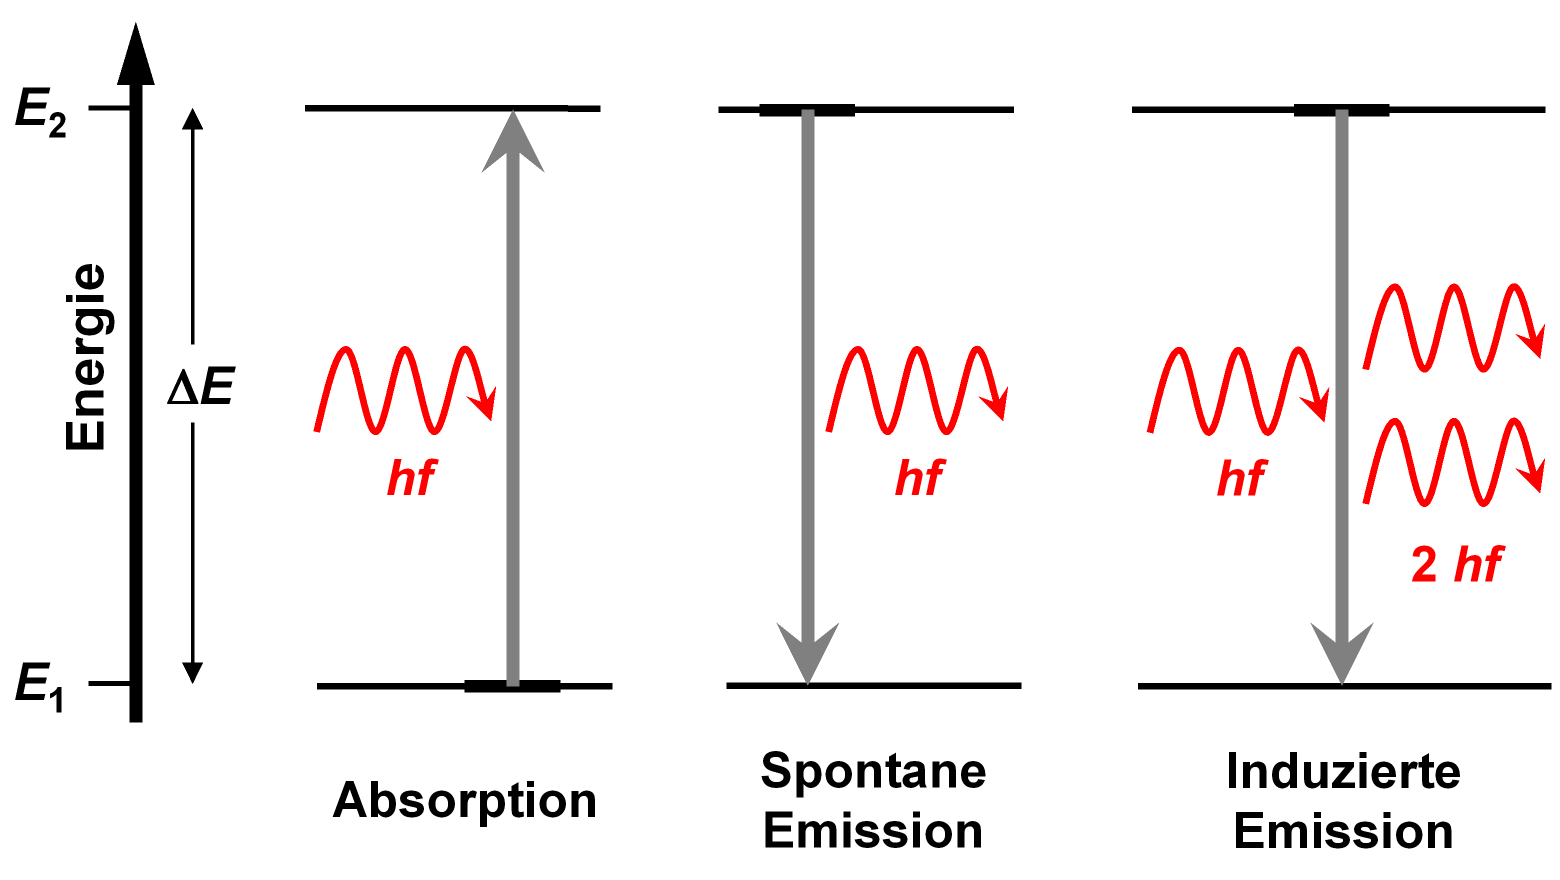
\includegraphics[width = \textwidth]{v61_bilder/emission.png}
    \caption{Schematische Darstellung der spontanen Emission (Mitte) und der stimulierten Emission (Rechts).}
    \label{fig:emission}
\end{figure}
\\Bei einem Laser werden diese emittierten Photonen auch gleichzeitig zur stimulierten Emission weiterer Photonen verwendet. Hierdurch
entsteht ein Selbstverstärkender Effekt. Damit das elektromagnetische Feld wieder auf das Medium trifft, wird ein Resonator verwendet.

\section{He-Ne Laser}

Der hier verwendete Lasers beinhaltet ein He-Ne Gasgemisch. Das Verhältnis der Atome beträgt etwa 5:1. Pro
Neonatom sind dementsprechend etwa 5 Heliumatome vorhanden. Die charakteristischen Eigenschaften des Lasers entstehen hier ausschließlich
durch die Neonatome. Das Helium dient als Pumpgas. Die He-Atome werden stetig durch elektrische Entladung im Laserrohr angeregt.
Diese Entladung wird durch einen niedrigen Druck von $p = \qty{1}{\mathrm{Torr}}$ erreicht.\\
Die Pumpquelle ist notwendig, um eine Besetzungsinversion des Neongases hervorzurufen. Es sollen sich also mehr Atome in einem angeregten
Zustand befinden, als im Grundzustand. Im thermischen Gleichgewicht ist dies nicht der Fall. Ohne eine solche Besetzungsinversion ist die Wahrscheinlichkeit, dass ein vorher emittiertes
Photon lediglich wieder absorbiert wird höher, als die Wahrscheinlichkeit, dass dieses eine stimulierte Emission auslöst. Die stimulierte
Emission muss allerdings stattfinden, damit ein Selbstverstärkender Effekt des Lasers auftreten kann.
Diese Besetzungsinversion wird dadurch realisiert, dass die angeregten He-Atome ihre Energie durch elastische Stöße mit Neonatomen abgeben,
wodurch diese wiederum angeregt werden. \\
Die Neonatome werden in zwei Zustände angeregt. Einerseits der 5s-Zustand und andererseits der 4s-Zustand. Diese angeregten
Zustände fallen entweder in den 4p- (nur für 5s) oder den 3p-Zustand. Zu beobachten sind somit 3 spezifische Energien der Photonen.
Am intensivsten ist hier der 5s zu 3p Übergang. Der durch diesen Übergang emittierten Photonen haben eine Energie von 
$\Delta E = \qty{20.66}{\electronvolt} - \qty{18.70}{\electronvolt} = \qty{1.96}{\electronvolt}$, entsprechend einer 
Wellenlänge von $\lambda = \qty{632.8}{\nano\metre}$ und einer Frequenz von $\nu = \frac{c}{\lambda} \approx \qty{474}{\mega\hertz}$.
Die Übergänge im Heliumatom sind in \autoref{fig:helium} schematisch gezeigt.
\begin{figure}
    \centering
    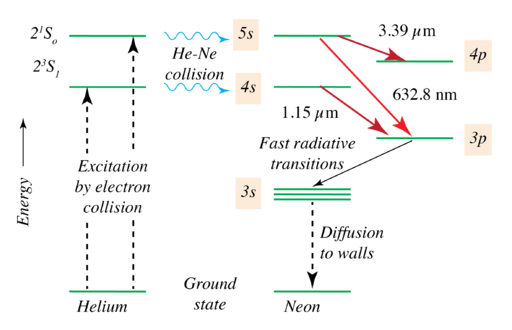
\includegraphics[width = \textwidth]{v61_bilder/helium.png}
    \caption{Schematische Darstellung der Energieübergänge des angeregten Heliumatoms.}
    \label{fig:helium}
\end{figure}
